\section{Engine\-Controller Class Reference}
\label{classEngineController}\index{EngineController@{EngineController}}
{\tt \#include $<$enginecontroller.h$>$}

Inheritance diagram for Engine\-Controller:\begin{figure}[H]
\begin{center}
\leavevmode
\includegraphics[width=96pt]{classEngineController__inherit__graph}
\end{center}
\end{figure}
Collaboration diagram for Engine\-Controller:\begin{figure}[H]
\begin{center}
\leavevmode
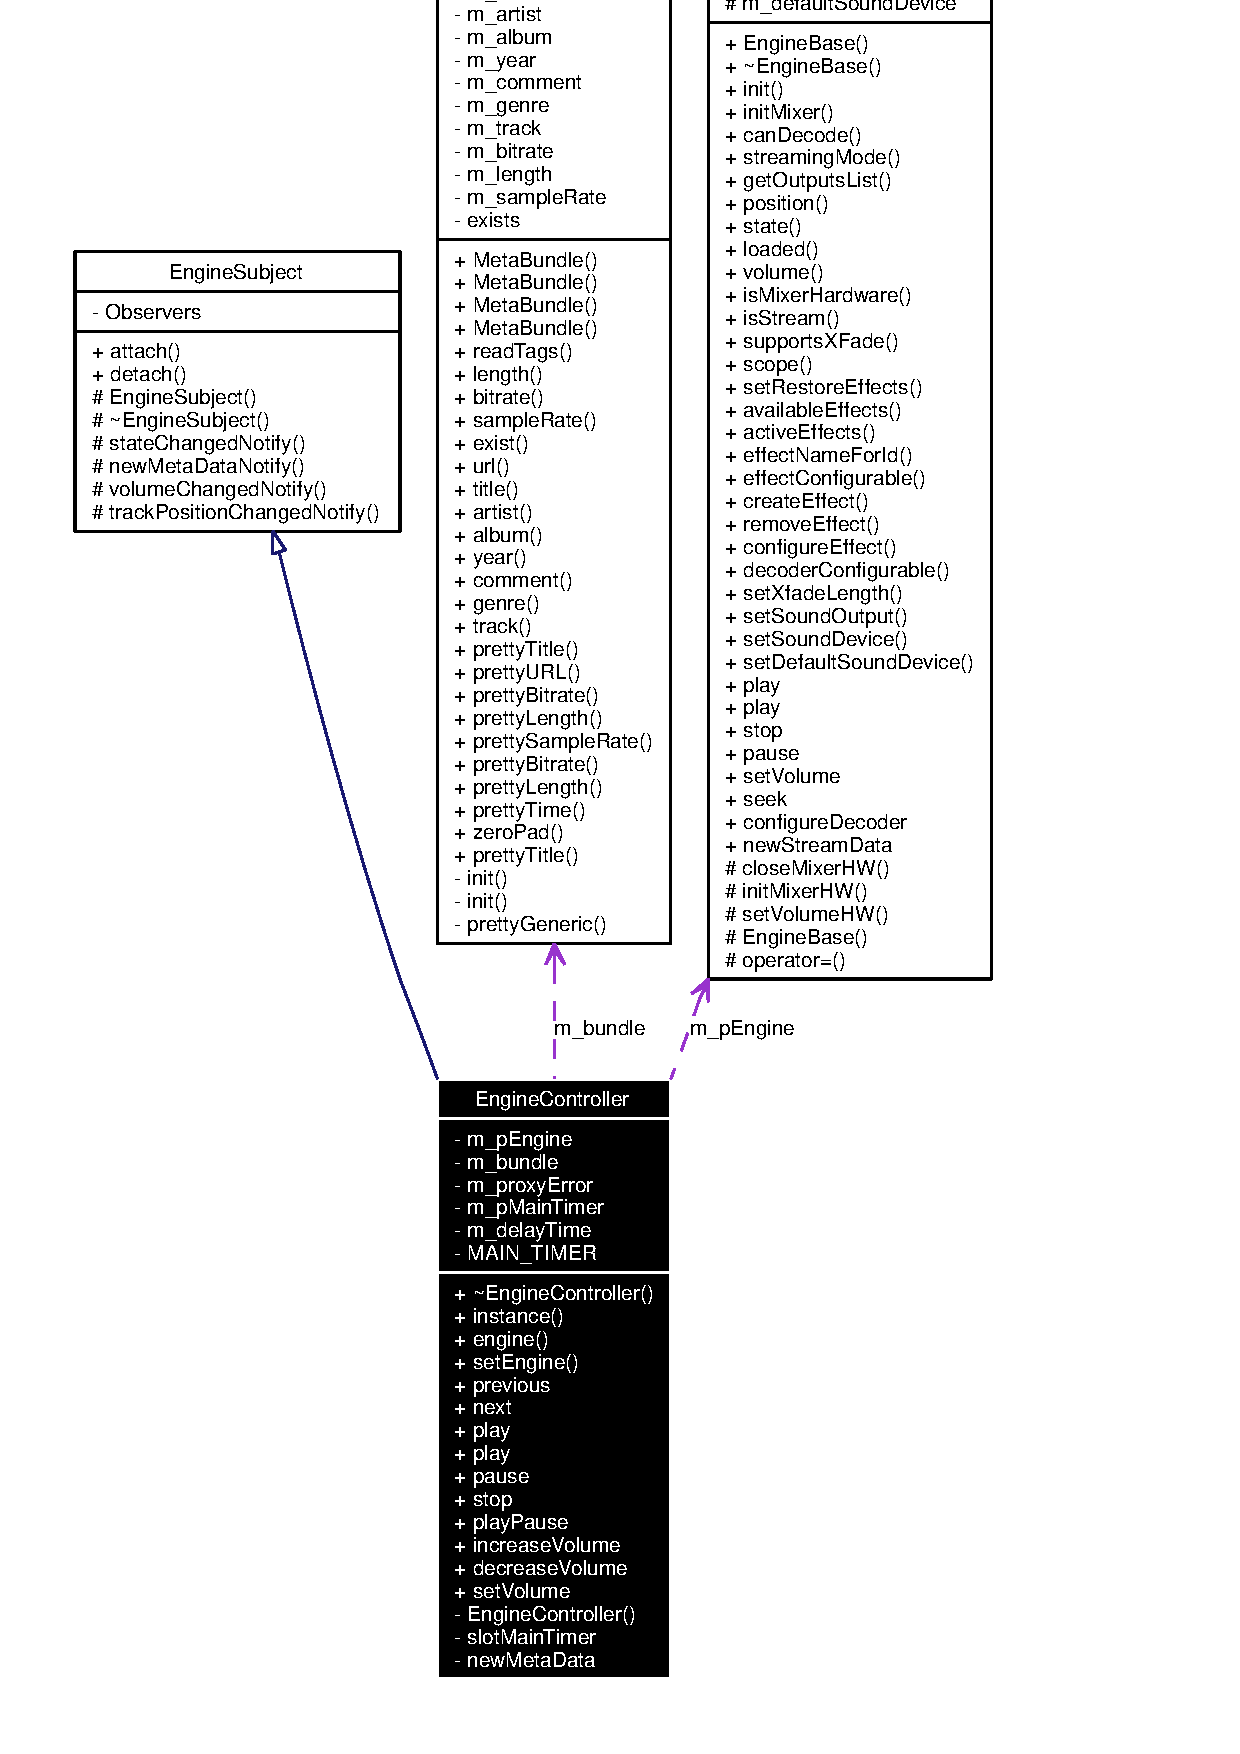
\includegraphics[width=238pt]{classEngineController__coll__graph}
\end{center}
\end{figure}


\subsection{Detailed Description}
This class captures amaro\-K specific behaviour for some common features. Accessing the engine directly is perfectly legal but on your own risk. TODO: Hide proxy stuff! 



Definition at line 33 of file enginecontroller.h.\subsection*{Public Slots}
\begin{CompactItemize}
\item 
void {\bf previous} ()
\item 
void {\bf next} ()
\item 
void {\bf play} (const {\bf Meta\-Bundle} \&bundle)
\item 
void {\bf play} (bool test, const {\bf Meta\-Bundle} \&bundle)
\item 
void {\bf pause} ()
\item 
void {\bf stop} ()
\item 
void {\bf play\-Pause} ()
\item 
int {\bf increase\-Volume} (int ticks=100/25)
\item 
int {\bf decrease\-Volume} (int ticks=100/25)
\item 
int {\bf set\-Volume} (int percent)
\end{CompactItemize}
\subsection*{Signals}
\begin{CompactItemize}
\item 
void {\bf order\-Next} ()
\item 
void {\bf order\-Previous} ()
\item 
void {\bf order\-Current} ()
\item 
void {\bf Track\-Position} (int)
\end{CompactItemize}
\subsection*{Public Member Functions}
\begin{CompactItemize}
\item 
virtual {\bf $\sim$Engine\-Controller} ()
\item 
void {\bf attach} ({\bf Engine\-Observer} $\ast$observer)
\item 
void {\bf detach} ({\bf Engine\-Observer} $\ast$observer)
\end{CompactItemize}
\subsection*{Static Public Member Functions}
\begin{CompactItemize}
\item 
{\bf Engine\-Controller} $\ast$ {\bf instance} ()
\item 
{\bf Engine\-Base} $\ast$ {\bf engine} ()
\item 
void {\bf set\-Engine} ({\bf Engine\-Base} $\ast$)
\end{CompactItemize}
\subsection*{Protected Member Functions}
\begin{CompactItemize}
\item 
void {\bf state\-Changed\-Notify} ({\bf Engine\-Base::Engine\-State})
\item 
void {\bf new\-Meta\-Data\-Notify} (const {\bf Meta\-Bundle} \&, bool)
\item 
void {\bf volume\-Changed\-Notify} (int)
\item 
void {\bf track\-Position\-Changed\-Notify} (long)
\end{CompactItemize}
\subsection*{Private Slots}
\begin{CompactItemize}
\item 
void {\bf slot\-Main\-Timer} ()
\item 
void {\bf new\-Meta\-Data} (const {\bf Meta\-Bundle} \&)
\end{CompactItemize}
\subsection*{Private Member Functions}
\begin{CompactItemize}
\item 
{\bf Engine\-Controller} ()
\end{CompactItemize}
\subsection*{Private Attributes}
\begin{CompactItemize}
\item 
{\bf Engine\-Base} $\ast$ {\bf m\_\-p\-Engine}
\item 
{\bf Meta\-Bundle} {\bf m\_\-bundle}
\item 
bool {\bf m\_\-proxy\-Error}
\item 
QTimer $\ast$ {\bf m\_\-p\-Main\-Timer}
\item 
long {\bf m\_\-delay\-Time}
\end{CompactItemize}
\subsection*{Static Private Attributes}
\begin{CompactItemize}
\item 
const int {\bf MAIN\_\-TIMER} = 150
\end{CompactItemize}


\subsection{Constructor \& Destructor Documentation}
\index{EngineController@{Engine\-Controller}!~EngineController@{$\sim$EngineController}}
\index{~EngineController@{$\sim$EngineController}!EngineController@{Engine\-Controller}}
\subsubsection{\setlength{\rightskip}{0pt plus 5cm}Engine\-Controller::$\sim${\bf Engine\-Controller} ()\hspace{0.3cm}{\tt  [virtual]}}\label{classEngineController_EngineControllera0}




Definition at line 77 of file enginecontroller.cpp.



\footnotesize\begin{verbatim}78 {
79 kdDebug() << k_funcinfo << endl;
80 }
\end{verbatim}\normalsize 
\index{EngineController@{Engine\-Controller}!EngineController@{EngineController}}
\index{EngineController@{EngineController}!EngineController@{Engine\-Controller}}
\subsubsection{\setlength{\rightskip}{0pt plus 5cm}Engine\-Controller::Engine\-Controller ()\hspace{0.3cm}{\tt  [private]}}\label{classEngineController_EngineControllerd0}




Definition at line 61 of file enginecontroller.cpp.

References dummy\-Engine, m\_\-p\-Engine, m\_\-p\-Main\-Timer, MAIN\_\-TIMER, Engine\-Base::set\-Volume(), and slot\-Main\-Timer().



\footnotesize\begin{verbatim}66     : m_pEngine( &dummyEngine ) //FIXME better would be a static member or something
67     , m_proxyError( false )
68     , m_pMainTimer( new QTimer( this ) )
69     , m_delayTime( 0 )
70 {
71     m_pEngine->setVolume( AmarokConfig::masterVolume() );
72 
73     connect( m_pMainTimer, SIGNAL( timeout() ), this, SLOT( slotMainTimer() ) );
74     m_pMainTimer->start( MAIN_TIMER );
75 }
\end{verbatim}\normalsize 


\subsection{Member Function Documentation}
\index{EngineController@{Engine\-Controller}!attach@{attach}}
\index{attach@{attach}!EngineController@{Engine\-Controller}}
\subsubsection{\setlength{\rightskip}{0pt plus 5cm}void Engine\-Subject::attach ({\bf Engine\-Observer} $\ast$ {\em observer})\hspace{0.3cm}{\tt  [inherited]}}\label{classEngineSubject_EngineSubjecta0}




Definition at line 92 of file engineobserver.cpp.

References Engine\-Subject::Observers.



\footnotesize\begin{verbatim}93 {
94     if( !observer || Observers.find( observer ) != -1 )
95         return;
96     Observers.append( observer );
97 }
\end{verbatim}\normalsize 
\index{EngineController@{Engine\-Controller}!decreaseVolume@{decreaseVolume}}
\index{decreaseVolume@{decreaseVolume}!EngineController@{Engine\-Controller}}
\subsubsection{\setlength{\rightskip}{0pt plus 5cm}int Engine\-Controller::decrease\-Volume (int {\em ticks} = 100/25)\hspace{0.3cm}{\tt  [slot]}}\label{classEngineController_EngineControlleri8}




Definition at line 180 of file enginecontroller.cpp.

References m\_\-p\-Engine, set\-Volume(), and Engine\-Base::volume().



\footnotesize\begin{verbatim}181 {
182     return setVolume( m_pEngine->volume() - ticks );
183 }
\end{verbatim}\normalsize 
\index{EngineController@{Engine\-Controller}!detach@{detach}}
\index{detach@{detach}!EngineController@{Engine\-Controller}}
\subsubsection{\setlength{\rightskip}{0pt plus 5cm}void Engine\-Subject::detach ({\bf Engine\-Observer} $\ast$ {\em observer})\hspace{0.3cm}{\tt  [inherited]}}\label{classEngineSubject_EngineSubjecta1}




Definition at line 100 of file engineobserver.cpp.

References Engine\-Subject::Observers.



\footnotesize\begin{verbatim}101 {
102     if( Observers.find( observer ) != -1 ) Observers.remove();
103 }
\end{verbatim}\normalsize 
\index{EngineController@{Engine\-Controller}!engine@{engine}}
\index{engine@{engine}!EngineController@{Engine\-Controller}}
\subsubsection{\setlength{\rightskip}{0pt plus 5cm}{\bf Engine\-Base}$\ast$ Engine\-Controller::engine ()\hspace{0.3cm}{\tt  [inline, static]}}\label{classEngineController_EngineControllere1}




Definition at line 43 of file enginecontroller.h.

References instance(), and m\_\-p\-Engine.

Referenced by Analyzer::Base$<$ W $>$::draw\-Frame(), and Myplayer::handle\-Slider().



\footnotesize\begin{verbatim}43 { return instance()->m_pEngine; }
\end{verbatim}\normalsize 


Here is the call graph for this function:\begin{figure}[H]
\begin{center}
\leavevmode
\includegraphics[width=166pt]{classEngineController_EngineControllere1_cgraph}
\end{center}
\end{figure}
\index{EngineController@{Engine\-Controller}!increaseVolume@{increaseVolume}}
\index{increaseVolume@{increaseVolume}!EngineController@{Engine\-Controller}}
\subsubsection{\setlength{\rightskip}{0pt plus 5cm}int Engine\-Controller::increase\-Volume (int {\em ticks} = 100/25)\hspace{0.3cm}{\tt  [slot]}}\label{classEngineController_EngineControlleri7}




Definition at line 173 of file enginecontroller.cpp.

References m\_\-p\-Engine, set\-Volume(), and Engine\-Base::volume().



\footnotesize\begin{verbatim}174 {
175     return setVolume( m_pEngine->volume() + ticks );
176 }
\end{verbatim}\normalsize 
\index{EngineController@{Engine\-Controller}!instance@{instance}}
\index{instance@{instance}!EngineController@{Engine\-Controller}}
\subsubsection{\setlength{\rightskip}{0pt plus 5cm}{\bf Engine\-Controller} $\ast$ Engine\-Controller::instance ()\hspace{0.3cm}{\tt  [static]}}\label{classEngineController_EngineControllere0}




Definition at line 53 of file enginecontroller.cpp.

Referenced by engine(), Myplayer::handle\-Next(), Myplayer::handle\-Previous(), Myplayer::Myplayer(), Myplayer::next(), Myplayer::pause(), Myplayer::play(), play(), Myplayer::previous(), set\-Engine(), Myplayer::set\-Volume(), and Myplayer::stop().



\footnotesize\begin{verbatim}54 {
55     //will only be instantiated the first time this function is called
56     static EngineController Instance;
57 
58     return &Instance;
59 }
\end{verbatim}\normalsize 
\index{EngineController@{Engine\-Controller}!newMetaData@{newMetaData}}
\index{newMetaData@{newMetaData}!EngineController@{Engine\-Controller}}
\subsubsection{\setlength{\rightskip}{0pt plus 5cm}void Engine\-Controller::new\-Meta\-Data (const {\bf Meta\-Bundle} \&)\hspace{0.3cm}{\tt  [inline, private, slot]}}\label{classEngineController_EngineControllerk1}




Definition at line 211 of file enginecontroller.cpp.



\footnotesize\begin{verbatim}212 {
213 /*    m_bundle = bundle;
214 
215 //    newMetaDataNotify( m_bundle, false  );*/
216 }
\end{verbatim}\normalsize 
\index{EngineController@{Engine\-Controller}!newMetaDataNotify@{newMetaDataNotify}}
\index{newMetaDataNotify@{newMetaDataNotify}!EngineController@{Engine\-Controller}}
\subsubsection{\setlength{\rightskip}{0pt plus 5cm}void Engine\-Subject::new\-Meta\-Data\-Notify (const {\bf Meta\-Bundle} \&, bool)\hspace{0.3cm}{\tt  [protected, inherited]}}\label{classEngineSubject_EngineSubjectb3}




Definition at line 56 of file engineobserver.cpp.

References Engine\-Observer::engine\-New\-Meta\-Data(), and Engine\-Subject::Observers.

Referenced by play().



\footnotesize\begin{verbatim}57 {
58     QPtrListIterator<EngineObserver> it( Observers );
59     EngineObserver *observer;
60     while( ( observer = it.current() ) != 0 )
61     {
62         ++it;
63         observer->engineNewMetaData( bundle, trackChanged );
64     }
65 }
\end{verbatim}\normalsize 


Here is the call graph for this function:\begin{figure}[H]
\begin{center}
\leavevmode
\includegraphics[width=217pt]{classEngineSubject_EngineSubjectb3_cgraph}
\end{center}
\end{figure}
\index{EngineController@{Engine\-Controller}!next@{next}}
\index{next@{next}!EngineController@{Engine\-Controller}}
\subsubsection{\setlength{\rightskip}{0pt plus 5cm}void Engine\-Controller::next ()\hspace{0.3cm}{\tt  [slot]}}\label{classEngineController_EngineControlleri1}




Definition at line 90 of file enginecontroller.cpp.

References order\-Next().

Referenced by Myplayer::next(), and slot\-Main\-Timer().



\footnotesize\begin{verbatim}91 {
92     kdDebug() << "EngineController->next" << endl;
93     emit orderNext();
94 }
\end{verbatim}\normalsize 
\index{EngineController@{Engine\-Controller}!orderCurrent@{orderCurrent}}
\index{orderCurrent@{orderCurrent}!EngineController@{Engine\-Controller}}
\subsubsection{\setlength{\rightskip}{0pt plus 5cm}void Engine\-Controller::order\-Current ()\hspace{0.3cm}{\tt  [signal]}}\label{classEngineController_EngineControllerl2}




Definition at line 161 of file enginecontroller.moc.



\footnotesize\begin{verbatim}162 {
163     activate_signal( staticMetaObject()->signalOffset() + 2 );
164 }
\end{verbatim}\normalsize 
\index{EngineController@{Engine\-Controller}!orderNext@{orderNext}}
\index{orderNext@{orderNext}!EngineController@{Engine\-Controller}}
\subsubsection{\setlength{\rightskip}{0pt plus 5cm}void Engine\-Controller::order\-Next ()\hspace{0.3cm}{\tt  [signal]}}\label{classEngineController_EngineControllerl0}




Definition at line 149 of file enginecontroller.moc.

Referenced by next().



\footnotesize\begin{verbatim}150 {
151     activate_signal( staticMetaObject()->signalOffset() + 0 );
152 }
\end{verbatim}\normalsize 
\index{EngineController@{Engine\-Controller}!orderPrevious@{orderPrevious}}
\index{orderPrevious@{orderPrevious}!EngineController@{Engine\-Controller}}
\subsubsection{\setlength{\rightskip}{0pt plus 5cm}void Engine\-Controller::order\-Previous ()\hspace{0.3cm}{\tt  [signal]}}\label{classEngineController_EngineControllerl1}




Definition at line 155 of file enginecontroller.moc.

Referenced by previous().



\footnotesize\begin{verbatim}156 {
157     activate_signal( staticMetaObject()->signalOffset() + 1 );
158 }
\end{verbatim}\normalsize 
\index{EngineController@{Engine\-Controller}!pause@{pause}}
\index{pause@{pause}!EngineController@{Engine\-Controller}}
\subsubsection{\setlength{\rightskip}{0pt plus 5cm}void Engine\-Controller::pause ()\hspace{0.3cm}{\tt  [slot]}}\label{classEngineController_EngineControlleri4}




Definition at line 150 of file enginecontroller.cpp.

References Engine\-Base::loaded(), m\_\-p\-Engine, Engine\-Base::pause(), Engine\-Base::play(), Engine\-Base::state(), and Engine\-Subject::state\-Changed\-Notify().

Referenced by Myplayer::pause(), and play().



\footnotesize\begin{verbatim}151 {
152     if ( m_pEngine->loaded() )
153     {
154         if ( m_pEngine->state() == EngineBase::Paused )
155             m_pEngine->play();
156         else
157             m_pEngine->pause();
158         stateChangedNotify( m_pEngine->state() );
159     }
160 }
\end{verbatim}\normalsize 
\index{EngineController@{Engine\-Controller}!play@{play}}
\index{play@{play}!EngineController@{Engine\-Controller}}
\subsubsection{\setlength{\rightskip}{0pt plus 5cm}void Engine\-Controller::play (bool {\em test}, const {\bf Meta\-Bundle} \& {\em bundle})\hspace{0.3cm}{\tt  [slot]}}\label{classEngineController_EngineControlleri3}




Definition at line 136 of file enginecontroller.cpp.

References m\_\-p\-Engine, Engine\-Subject::new\-Meta\-Data\-Notify(), Engine\-Base::play(), Engine\-Subject::state\-Changed\-Notify(), and Meta\-Bundle::url().



\footnotesize\begin{verbatim}137 {
138         const KURL &trackurl = bundle.url();    
139         kdDebug() << "[enginecontroller]SoundSystem: " << bundle.url() << endl;
140         m_pEngine->play( trackurl );    
141 
142    //  kdDebug() << "[engine] It's Playing: " << bundle.track() << endl;
143 
144     stateChangedNotify( EngineBase::Playing );
145     newMetaDataNotify( bundle, true /* track change */ );
146       
147 }
\end{verbatim}\normalsize 
\index{EngineController@{Engine\-Controller}!play@{play}}
\index{play@{play}!EngineController@{Engine\-Controller}}
\subsubsection{\setlength{\rightskip}{0pt plus 5cm}void Engine\-Controller::play (const {\bf Meta\-Bundle} \& {\em bundle})\hspace{0.3cm}{\tt  [slot]}}\label{classEngineController_EngineControlleri2}




Definition at line 111 of file enginecontroller.cpp.

References instance(), m\_\-p\-Engine, pause(), Engine\-Base::play(), Engine\-Base::state(), and Engine\-Subject::state\-Changed\-Notify().

Referenced by Myplayer::handle\-Next(), Myplayer::handle\-Previous(), and Myplayer::play().



\footnotesize\begin{verbatim}112 {
113 qWarning("[EngineController::play]");
114     if ( m_pEngine->state() == EngineBase::Paused )
115     {
116         m_pEngine->play();
117         stateChangedNotify( EngineBase::Playing );
118 qWarning("Pause->play");        
119     }
120     else if( m_pEngine->state() == EngineBase::Playing )
121     {
122         EngineController::instance()->pause();  
123         
124 qWarning("play->pause");        
125     }
126     else 
127     {
128          EngineController::instance()->play(true,bundle);
129         
130 qWarning("other situation");    
131     }   
132 //        emit orderCurrent(); // keep currenttrack to avoid signal?
133 }
\end{verbatim}\normalsize 
\index{EngineController@{Engine\-Controller}!playPause@{playPause}}
\index{playPause@{playPause}!EngineController@{Engine\-Controller}}
\subsubsection{\setlength{\rightskip}{0pt plus 5cm}void Engine\-Controller::play\-Pause ()\hspace{0.3cm}{\tt  [slot]}}\label{classEngineController_EngineControlleri6}




Definition at line 98 of file enginecontroller.cpp.



\footnotesize\begin{verbatim}99 {
100 /*    //this is used by the TrayIcon and PlayPauseAction
101 
102     if( m_pEngine->state() == EngineBase::Playing )
103     {
104         pause();
105     }
106     else play();*/
107 }
\end{verbatim}\normalsize 
\index{EngineController@{Engine\-Controller}!previous@{previous}}
\index{previous@{previous}!EngineController@{Engine\-Controller}}
\subsubsection{\setlength{\rightskip}{0pt plus 5cm}void Engine\-Controller::previous ()\hspace{0.3cm}{\tt  [slot]}}\label{classEngineController_EngineControlleri0}




Definition at line 83 of file enginecontroller.cpp.

References order\-Previous().

Referenced by Myplayer::previous().



\footnotesize\begin{verbatim}84 {
85     emit orderPrevious();
86 }
\end{verbatim}\normalsize 
\index{EngineController@{Engine\-Controller}!setEngine@{setEngine}}
\index{setEngine@{setEngine}!EngineController@{Engine\-Controller}}
\subsubsection{\setlength{\rightskip}{0pt plus 5cm}void Engine\-Controller::set\-Engine ({\bf Engine\-Base} $\ast$)\hspace{0.3cm}{\tt  [static]}}\label{classEngineController_EngineControllere2}




Definition at line 186 of file enginecontroller.cpp.

References instance(), and m\_\-p\-Engine.

Referenced by Myplayer::Myplayer().



\footnotesize\begin{verbatim}187 {
188     instance()->m_pEngine = engine;
189     kdDebug() << "[enginecontroller]engine: " << engine << endl;
190     //NOTE many engine properties are only set in applySettings
191 }
\end{verbatim}\normalsize 


Here is the call graph for this function:\begin{figure}[H]
\begin{center}
\leavevmode
\includegraphics[width=174pt]{classEngineController_EngineControllere2_cgraph}
\end{center}
\end{figure}
\index{EngineController@{Engine\-Controller}!setVolume@{setVolume}}
\index{setVolume@{setVolume}!EngineController@{Engine\-Controller}}
\subsubsection{\setlength{\rightskip}{0pt plus 5cm}int Engine\-Controller::set\-Volume (int {\em percent})\hspace{0.3cm}{\tt  [slot]}}\label{classEngineController_EngineControlleri9}




Definition at line 193 of file enginecontroller.cpp.

References m\_\-p\-Engine, Amarok\-Config::set\-Master\-Volume(), Engine\-Base::set\-Volume(), Engine\-Base::volume(), and Engine\-Subject::volume\-Changed\-Notify().

Referenced by decrease\-Volume(), increase\-Volume(), and Myplayer::set\-Volume().



\footnotesize\begin{verbatim}194 {
195     if( percent < 0 ) percent = 0; //can't make uint as all signals use int and slot has to match
196     if( percent > 100 ) percent = 100;
197 
198     if( percent != m_pEngine->volume() )
199     {
200         AmarokConfig::setMasterVolume( percent );
201 
202         m_pEngine->setVolume( percent );
203 
204         volumeChangedNotify( percent );
205     }
206 
207     return m_pEngine->volume();
208 }
\end{verbatim}\normalsize 
\index{EngineController@{Engine\-Controller}!slotMainTimer@{slotMainTimer}}
\index{slotMainTimer@{slotMainTimer}!EngineController@{Engine\-Controller}}
\subsubsection{\setlength{\rightskip}{0pt plus 5cm}void Engine\-Controller::slot\-Main\-Timer ()\hspace{0.3cm}{\tt  [inline, private, slot]}}\label{classEngineController_EngineControllerk0}




Definition at line 220 of file enginecontroller.cpp.

References Amarok\-Config::crossfade(), Amarok\-Config::crossfade\-Length(), Engine\-Base::is\-Stream(), Meta\-Bundle::length(), m\_\-bundle, m\_\-delay\-Time, m\_\-p\-Engine, MAIN\_\-TIMER, next(), Engine\-Base::position(), Engine\-Base::state(), Engine\-Base::supports\-XFade(), Amarok\-Config::track\-Delay\-Length(), Track\-Position(), and Engine\-Subject::track\-Position\-Changed\-Notify().

Referenced by Engine\-Controller().



\footnotesize\begin{verbatim}221 {
222     if( m_pEngine->state() == EngineBase::Empty ) return;
223     const uint position = m_pEngine->position();
224     const uint length   = m_bundle.length() * 1000;
225 
226     trackPositionChangedNotify( position );
227 
228     // check if track has ended or is broken
229     if ( m_pEngine->state() == EngineBase::Idle )
230     {
231         kdDebug() << k_funcinfo << "Idle detected. Skipping track.\n";
232 
233         if ( AmarokConfig::trackDelayLength() > 0 ) //this can occur syncronously to XFade and not be fatal
234         {
235             //delay before start of next track, without freezing the app
236             m_delayTime += MAIN_TIMER;
237             if ( m_delayTime >= AmarokConfig::trackDelayLength() )
238             {
239                 m_delayTime = 0;
240                 next();
241             }
242         }
243         else
244             next();
245     }
246     // Crossfading
247     else if ( ( AmarokConfig::crossfade() ) &&
248               ( m_pEngine->supportsXFade() ) &&
249               ( !m_pEngine->isStream() ) &&
250               ( length ) &&
251               ( length - position < (uint)AmarokConfig::crossfadeLength() )  )
252     {
253         kdDebug() << k_funcinfo << "Crossfading to next track.\n";
254         next();
255     }
256     emit TrackPosition(position/1000);
257 }
\end{verbatim}\normalsize 
\index{EngineController@{Engine\-Controller}!stateChangedNotify@{stateChangedNotify}}
\index{stateChangedNotify@{stateChangedNotify}!EngineController@{Engine\-Controller}}
\subsubsection{\setlength{\rightskip}{0pt plus 5cm}void Engine\-Subject::state\-Changed\-Notify ({\bf Engine\-Base::Engine\-State})\hspace{0.3cm}{\tt  [protected, inherited]}}\label{classEngineSubject_EngineSubjectb2}




Definition at line 44 of file engineobserver.cpp.

References Engine\-Observer::engine\-State\-Changed(), and Engine\-Subject::Observers.

Referenced by pause(), play(), and stop().



\footnotesize\begin{verbatim}45 {
46     QPtrListIterator<EngineObserver> it( Observers );
47     EngineObserver *observer;
48     while( ( observer = it.current() ) != 0 )
49     {
50         ++it;
51         observer->engineStateChanged( state );
52     }
53 }
\end{verbatim}\normalsize 


Here is the call graph for this function:\begin{figure}[H]
\begin{center}
\leavevmode
\includegraphics[width=217pt]{classEngineSubject_EngineSubjectb2_cgraph}
\end{center}
\end{figure}
\index{EngineController@{Engine\-Controller}!stop@{stop}}
\index{stop@{stop}!EngineController@{Engine\-Controller}}
\subsubsection{\setlength{\rightskip}{0pt plus 5cm}void Engine\-Controller::stop ()\hspace{0.3cm}{\tt  [slot]}}\label{classEngineController_EngineControlleri5}




Definition at line 164 of file enginecontroller.cpp.

References m\_\-p\-Engine, Engine\-Base::state(), Engine\-Subject::state\-Changed\-Notify(), and Engine\-Base::stop().

Referenced by Myplayer::handle\-Next(), Myplayer::next(), Myplayer::play(), Myplayer::previous(), and Myplayer::stop().



\footnotesize\begin{verbatim}165 {
166 /*    m_bundle = MetaBundle(); */
167     m_pEngine->stop();
168     stateChangedNotify( m_pEngine->state() );  
169 }
\end{verbatim}\normalsize 
\index{EngineController@{Engine\-Controller}!TrackPosition@{TrackPosition}}
\index{TrackPosition@{TrackPosition}!EngineController@{Engine\-Controller}}
\subsubsection{\setlength{\rightskip}{0pt plus 5cm}void Engine\-Controller::Track\-Position (int)\hspace{0.3cm}{\tt  [signal]}}\label{classEngineController_EngineControllerl3}




Definition at line 167 of file enginecontroller.moc.

Referenced by slot\-Main\-Timer().



\footnotesize\begin{verbatim}168 {
169     activate_signal( staticMetaObject()->signalOffset() + 3, t0 );
170 }
\end{verbatim}\normalsize 
\index{EngineController@{Engine\-Controller}!trackPositionChangedNotify@{trackPositionChangedNotify}}
\index{trackPositionChangedNotify@{trackPositionChangedNotify}!EngineController@{Engine\-Controller}}
\subsubsection{\setlength{\rightskip}{0pt plus 5cm}void Engine\-Subject::track\-Position\-Changed\-Notify (long)\hspace{0.3cm}{\tt  [protected, inherited]}}\label{classEngineSubject_EngineSubjectb5}




Definition at line 80 of file engineobserver.cpp.

References Engine\-Observer::engine\-Track\-Position\-Changed(), and Engine\-Subject::Observers.

Referenced by slot\-Main\-Timer().



\footnotesize\begin{verbatim}81 {
82     QPtrListIterator<EngineObserver> it( Observers );
83     EngineObserver *observer;
84     while( ( observer = it.current() ) != 0 )
85     {
86         ++it;
87         observer->engineTrackPositionChanged( position );
88     }
89 }
\end{verbatim}\normalsize 


Here is the call graph for this function:\begin{figure}[H]
\begin{center}
\leavevmode
\includegraphics[width=253pt]{classEngineSubject_EngineSubjectb5_cgraph}
\end{center}
\end{figure}
\index{EngineController@{Engine\-Controller}!volumeChangedNotify@{volumeChangedNotify}}
\index{volumeChangedNotify@{volumeChangedNotify}!EngineController@{Engine\-Controller}}
\subsubsection{\setlength{\rightskip}{0pt plus 5cm}void Engine\-Subject::volume\-Changed\-Notify (int)\hspace{0.3cm}{\tt  [protected, inherited]}}\label{classEngineSubject_EngineSubjectb4}




Definition at line 68 of file engineobserver.cpp.

References Engine\-Observer::engine\-Volume\-Changed(), and Engine\-Subject::Observers.

Referenced by set\-Volume().



\footnotesize\begin{verbatim}69 {
70     QPtrListIterator<EngineObserver> it( Observers );
71     EngineObserver *observer;
72     while( ( observer = it.current() ) != 0 )
73     {
74         ++it;
75         observer->engineVolumeChanged( percent );
76     }
77 }
\end{verbatim}\normalsize 


Here is the call graph for this function:\begin{figure}[H]
\begin{center}
\leavevmode
\includegraphics[width=227pt]{classEngineSubject_EngineSubjectb4_cgraph}
\end{center}
\end{figure}


\subsection{Member Data Documentation}
\index{EngineController@{Engine\-Controller}!m_bundle@{m\_\-bundle}}
\index{m_bundle@{m\_\-bundle}!EngineController@{Engine\-Controller}}
\subsubsection{\setlength{\rightskip}{0pt plus 5cm}{\bf Meta\-Bundle} {\bf Engine\-Controller::m\_\-bundle}\hspace{0.3cm}{\tt  [private]}}\label{classEngineController_EngineControllerr1}




Definition at line 81 of file enginecontroller.h.

Referenced by slot\-Main\-Timer().\index{EngineController@{Engine\-Controller}!m_delayTime@{m\_\-delayTime}}
\index{m_delayTime@{m\_\-delayTime}!EngineController@{Engine\-Controller}}
\subsubsection{\setlength{\rightskip}{0pt plus 5cm}long {\bf Engine\-Controller::m\_\-delay\-Time}\hspace{0.3cm}{\tt  [private]}}\label{classEngineController_EngineControllerr4}




Definition at line 84 of file enginecontroller.h.

Referenced by slot\-Main\-Timer().\index{EngineController@{Engine\-Controller}!m_pEngine@{m\_\-pEngine}}
\index{m_pEngine@{m\_\-pEngine}!EngineController@{Engine\-Controller}}
\subsubsection{\setlength{\rightskip}{0pt plus 5cm}{\bf Engine\-Base}$\ast$ {\bf Engine\-Controller::m\_\-p\-Engine}\hspace{0.3cm}{\tt  [private]}}\label{classEngineController_EngineControllerr0}




Definition at line 80 of file enginecontroller.h.

Referenced by decrease\-Volume(), engine(), Engine\-Controller(), increase\-Volume(), pause(), play(), set\-Engine(), set\-Volume(), slot\-Main\-Timer(), and stop().\index{EngineController@{Engine\-Controller}!m_pMainTimer@{m\_\-pMainTimer}}
\index{m_pMainTimer@{m\_\-pMainTimer}!EngineController@{Engine\-Controller}}
\subsubsection{\setlength{\rightskip}{0pt plus 5cm}QTimer$\ast$ {\bf Engine\-Controller::m\_\-p\-Main\-Timer}\hspace{0.3cm}{\tt  [private]}}\label{classEngineController_EngineControllerr3}




Definition at line 83 of file enginecontroller.h.

Referenced by Engine\-Controller().\index{EngineController@{Engine\-Controller}!m_proxyError@{m\_\-proxyError}}
\index{m_proxyError@{m\_\-proxyError}!EngineController@{Engine\-Controller}}
\subsubsection{\setlength{\rightskip}{0pt plus 5cm}bool {\bf Engine\-Controller::m\_\-proxy\-Error}\hspace{0.3cm}{\tt  [private]}}\label{classEngineController_EngineControllerr2}




Definition at line 82 of file enginecontroller.h.\index{EngineController@{Engine\-Controller}!MAIN_TIMER@{MAIN\_\-TIMER}}
\index{MAIN_TIMER@{MAIN\_\-TIMER}!EngineController@{Engine\-Controller}}
\subsubsection{\setlength{\rightskip}{0pt plus 5cm}const int {\bf Engine\-Controller::MAIN\_\-TIMER} = 150\hspace{0.3cm}{\tt  [static, private]}}\label{classEngineController_EngineControllerv0}




Definition at line 78 of file enginecontroller.h.

Referenced by Engine\-Controller(), and slot\-Main\-Timer().

The documentation for this class was generated from the following files:\begin{CompactItemize}
\item 
{\bf enginecontroller.h}\item 
{\bf enginecontroller.moc}\item 
{\bf enginecontroller.cpp}\end{CompactItemize}
